\section{Management Summary}

\subsection{Roles and Responsabilities}
\begin{table}[h!]
	\begin{tabular}{p{5cm}p{11cm}}
		 \parbox[c]{1em}{ 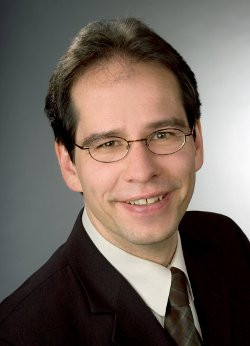
\includegraphics[width=1in]{oliver} }  & \textbf{Advisor:}\quad  Prof. Oliver Augenstein, Professor of Mathematics \\
				 & \\ %Empty row
		 \parbox[c]{1em}{ 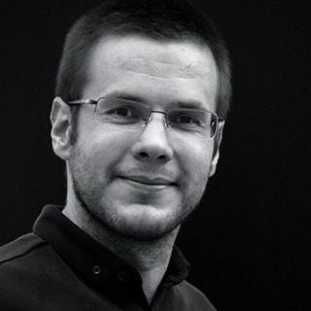
\includegraphics[width=1in]{roberto} }  & \textbf{Project Developer:}\quad  Roberto Cuervo, HSR Computer Sciences Student\\
		 		 & \\ %Empty row
		 \parbox[c]{1em}{ 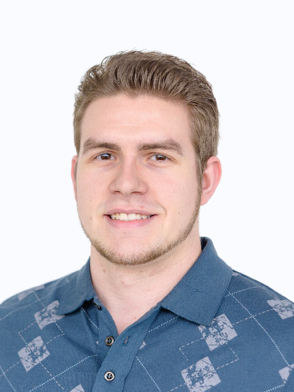
\includegraphics[width=1in]{konrad} }  & \textbf{Project Developer:}\quad  Konrad H\"opli, HSR Computer Sciences Student \\
	\end{tabular}
\end{table}



\subsection{Start Position}
 
The Clinic for Masticatory Disorders of the University of Zurich employs a mixture of proprietary software (\gls{tmjviewer}), hardware (3D Cameras System, \gls{optis}) and components made with other commercial software (MatLab, among others) in order to display the jaw bones of a patient combined with its recorded movement in a 3D animation for medical analysis. Working with all these different applications/components, different file formats and various manual inputs is time consuming, error-prone and does not allow real-time interaction with the patient. 

Due to the lack of feedback in real-time, it takes an extended period of time until the doctors can see and analyse the recordings of a patient. In the case of a mistake by the patient him-/herself during the recording or in the processing of the data afterwards, another appointment might need to be scheduled essentially starting the process all over again and resulting in an unpleasant experience for both parties involved.

As a result, the Clinic desires an application with the goal of eventually unifying all the steps involved and adding the ability to support real-time display and therewith immediate feedback for the patient. While this represents the basic idea behind this project, the resulting software of it was not intended to be fully implemented within the given timeframe.


\subsection{Approach}

In the very beginning of the project and even before our first meeting with the involved people of the Clinic for Masticatory Disorders, we had to familiarize ourselves with the \gls{opengl} technology that was going to be used for the graphical components of this project. We did so by consuming literature on the topic and then developing a prototype based on a suited tutorial recommended by Prof. Augenstein.

After these first steps into the complex domain, we scheduled a meeting at the Clinic in order to get to know all the people involved, but also the tools and technology already in use. Due to the complexity of the solution in place and various proprietary components and file formats, we quickly realized that we would not be able to determine what is feasible over the course of this project off the bat and thus an agile approach would be best suited for this project.

We then set the first goal for our interim presentation to get a basic application running that would display the bones of a patient with the recorded motion using a set of demonstration data provided. After reaching this first goal, we identified the next most desirable features with all the people and ended up deriving from the initial focus on the real-time capability since the progress was much more sluggish than expected. The root causes for this form of progress was both caused by the lack of experience on the side of the developers, but also the lack of documentation and clear information on the side of the Clinic.

\subsection{Results}
The results of this thesis consist of:
\begin{itemize}
	\item  An application which meets most of the essential requirements, but is not sufficient for productive use. 
	\item  Documentation covering an introduction into OpenGL, the development of this project as well as the mathematical foundations used therein
\end{itemize}
The resulting application ended up much more basic than initially hoped and planned. However, the derivation from the initially defined goals for the developed application was deemed necessary due to the underlying complexity of the domain and absence of good information as well as documentation on the components in use.

 
\subsection{Conclusion}
The results of this project are not suitable for a productive environment, but both the documentation and the software created can serve as a very good foundation for future developments in this area. The graphical part of the application was designed to be a standalone component of which individual features can be extracted with ease and the documentation does not just cover the course of this project, but also contain viable information that the students would have liked to have when they started out.
